\documentclass[a4paper, 11pt]{article}

\usepackage{parskip}
\usepackage{hyperref}
\hypersetup{ colorlinks, citecolor=green, filecolor=black, linkcolor=blue, urlcolor=blue } 

\usepackage{colortbl}

\usepackage{amsfonts}

\usepackage[left=2cm, right=2cm, top=2cm]{geometry}
\usepackage{float}
\usepackage{afterpage}
\usepackage{multirow}

\usepackage{gensymb}
\usepackage{amsmath}
\usepackage{graphicx}
\usepackage{enumitem}

\newcommand{\points}[1]{(\textbf{#1 marks}) }
\newcommand{\vecthree}[3]{\begin{pmatrix} #1 \\ #2 \\ #3 \end{pmatrix}}
\newcommand{\vecfour}[4]{\begin{pmatrix} #1 \\ #2 \\ #3 \\ #4\end{pmatrix}}
\newcommand{\mat}[1]{\boldsymbol { \mathsf{#1}} }

\DeclareMathOperator*{\argmax}{arg\,max}
\DeclareMathOperator*{\argmin}{arg\,min}
\newcommand{\norm}[1]{\lVert#1\rVert}
\newcommand{\R}{\mathbb{R}}

\definecolor{mycolor}{rgb}{0,0.6,0.5}

\title{Solutions - Group project 1\\CS340/MATH321 -- Geometrical modelling and numerical analysis}
\vspace{-10em}
\date{Fall 2019}
\author{Huda Feroz Ahmed, Mujtaba Rohani, Muhammad Ahmed}

\begin{document}
\maketitle  
\setlength{\parskip}{10pt}
\setlength{\parindent}{0pt}
\DeclareGraphicsExtensions{.pdf,.png,.gif,.jpg}

\section*{Solution of Question 1}
    
\begin{enumerate}[label=\alph*.]
    \item
    Solution of part a goes here.\\
    
    To find $\Vec{t}$, we have to differentiate the function $J$ w.r.t. to $\Vec{t}$.
    
    \begin{align}
        \frac{\partial J(\mat R,\Vec{t})}{\partial \Vec{t}} & = \frac{\partial}{\partial \Vec{t}} \left[ \sum_{i=1}^{n} \omega_i\norm{(\mat R\vec p_i+\vec t)-\vec q_i}^2 \right]
    \end{align}
    
    On the right hand side, we can take the partial derivative inside the summation. Also $\omega_i$ does not depend on $\vec t$ so it can be taken out as well. Also, this derivative must be set to $0$ to find stationary points.
    
    \begin{align}
         \sum_{i=1}^{n} \omega_i \frac{\partial}{\partial \Vec{t}} \left[ \norm{(\mat R\vec p_i+\vec t)-\vec q_i}^2 \right] = 0
    \end{align} 
    
    \begin{align}
         \sum_{i=1}^{n} \omega_i 2\times \left[ \norm{(\mat R\vec p_i+\vec t)-\vec q_i} \right] \frac{\partial}{\partial \Vec{t}} \left[ \norm{(\mat R\vec p_i+\vec t)-\vec q_i} \right] = 0
    \end{align}
    
    \begin{align}
         \sum_{i=1}^{n} \omega_i 2\times \left[ \norm{(\mat R\vec p_i+\vec t)-\vec q_i} \right] \frac{\partial}{\partial \Vec{t}} \left[ \norm{(\mat R\vec p_i+\vec t)-\vec q_i} \right] = 0
    \end{align}
    
    \begin{align}
         \sum_{i=1}^{n} \omega_i \times 2 \left[ \norm{(\mat R\vec p_i+\vec t)-\vec q_i} \right] \frac{\partial}{\partial \Vec{t}} \left[ \sqrt{\sum_{j=1}^d (\mat R p_{ij}+ t_j- q_{ij})^2} \right] = 0
    \end{align}
    
    Where,
    \begin{align} 
        \sqrt{\sum_{j=1}^d (\mat R p_ij+ t_j- q_ij)^2} = \norm{(\mat R\vec p_i+\vec t)-\vec q_i}
    \end{align}{}
    Where, $d$ is the dimension of $\vec p$ and $\vec q$.
    
    We know that,  $$\frac{d}{dx} (\sqrt{u}) = \frac{1}{2\sqrt{u}} \times \frac{du}{dx}$$
    
    Therefore, our expression becomes:
    
    \begin{align}
         0 &= \sum_{i=1}^{n} \omega_i \times 2 \left[ \norm{(\mat R\vec p_i+\vec t)-\vec q_i} \right] \times \frac{1}{2 \left[ \norm{(\mat R\vec p_i+\vec t)-\vec q_i} \right]} \frac{\partial}{\partial \Vec{t} } \left[ \sum_{j=1}^d (\mat R p_{ij}+ t_j- q_{ij})^2 \right]\\
         0 &= \sum_{i=1}^{n} \omega_i \left[ \sum_{j=1}^d \frac{\partial}{\partial \Vec{t} } (\mat R p_{ij}+ t_j- q_{ij})^2 \right] & = 0\\
         & \text{Using Chain rule,}\\
         0 &= \sum_{i=1}^{n} \omega_i \left[ \sum_{j=1}^d \times 2 (\mat R p_{ij}+ t_j - q_{ij}) \times (1) \right]\\
         0 &= \sum_{i=1}^{n} \omega_i  \times 2 (\mat R \vec p_i+ \vec t- \vec q_i)\\
         0 &= \sum_{i=1}^{n} \omega_i \mat R \vec p_i+ \sum_{i=1}^{n} \omega_i \vec t - \sum_{i=1}^{n} \omega_i \vec q_i\\
         \sum_{i=1}^{n} \omega_i \vec t &= \sum_{i=1}^{n} \omega_i \vec q_i - \sum_{i=1}^{n} \omega_i \mat R \vec p_i \\
         \vec t &= \frac{\sum_{i=1}^{n} \omega_i \vec q_i}{\sum_{i=1}^{n} \omega_i } - \mat R \frac{\sum_{i=1}^{n} \omega_i \vec p_i}{\sum_{i=1}^{n} \omega_i}
    \end{align}
    Where, $\frac{\sum_{i=1}^{n} \omega_i \vec q_i}{\sum_{i=1}^{n} \omega_i } = \vec q$ and $\frac{\sum_{i=1}^{n} \omega_i \vec p_i}{\sum_{i=1}^{n} \omega_i} = \vec p$ are the weighted centroids of the body $\mat Q$ and $\mat P$, respectively. Hence, the equation becomes,
    \begin{align}
        \vec t &= \vec q - \mat R \vec p
    \end{align}
    
    
    

    
    \item
    Solution of part b goes here.\\
    
    Substituting the value of $\vec t$ in function $J$:
    
    \begin{align}
  J(\mat R) &= \argmin\sum_{i=1}^{n}\omega_i\norm{\mat R\vec p_i+ \vec q - \mat R \vec p -\vec q_i}^2
    \end{align}
    
    \begin{align}
  J(\mat R) &= \argmin\sum_{i=1}^{n}\omega_i\norm{\mat R (\vec p_i - \vec p) - (\vec q -\vec q_i)}^2
    \end{align}
    
    We can take $\vec \alpha_i = \vec p_i - \vec p$ and $\vec \beta_i = \vec q_i - \vec q$. These $\alpha_i$ and $\beta_i$ are the directed vectors from the centroid to the vertices of the body. Therefore, equation becomes:
    
    \begin{align}
  J(\mat R) &= \argmin\sum_{i=1}^{n}\omega_i\norm{\mat R \alpha_i - \beta_i}^2 \label{18}
    \end{align}
    
    \item
    Solution of part c goes here.\\
    
    Eq \eqref{18} can be re-written in the form of inner vector product:
    
    \begin{align}
  J(\mat R) &= \argmin\sum_{i=1}^{n}\omega_i (\mat R \alpha_i - \beta_i)^T(\mat R \alpha_i - \beta_i)
    \end{align}
    
    \begin{align}
  J(\mat R) &= \argmin\sum_{i=1}^{n}\omega_i (\alpha_i^T \mat R^T - \beta_i^T)(\mat R \alpha_i - \beta_i)
    \end{align}
    
    \begin{align}
  J(\mat R) &= \argmin\sum_{i=1}^{n}\omega_i (\alpha_i^T \mat R^T \mat R \alpha_i - \beta_i^T \mat R \alpha_i -  \alpha_i^T \mat R^T \beta_i + \beta_i^T \beta_i )
    \end{align}
    
    \begin{align}
  J(\mat R) &= \argmin\sum_{i=1}^{n}\omega_i (\alpha_i^T \alpha_i - \beta_i^T \mat R \alpha_i -  \alpha_i^T \mat R^T \beta_i + \beta_i^T \beta_i )\label{22}
    \end{align}
    
    Here, $\beta_i^T \mat R \alpha_i$ is scalar quantity so it is is equal to its transpose.
    
    
    
    $$\beta_i^T \mat R \alpha_i = (\beta_i^T \mat R \alpha_i)^T = \alpha_i^T \mat R^T \beta_i$$
    
    Hence the equation \eqref{22} becomes,
    \begin{align}
        J(\mat R) &= \argmin\sum_{i=1}^{n}\omega_i (\alpha_i^T \alpha_i - 2\beta_i^T \mat R \alpha_i + \beta_i^T \beta_i )
    \end{align}
    
    Since the first and last term in the equation does not depend on $\mat R$, they can be ignored while minimizing the function $J(\mat R)$. Also, note the negative sign with $\beta_i^T \mat R \alpha_i$, which indicates that maximizing this term would minimize the function $J(\mat R)$. \cite{rigid body}
    \begin{align}
        J(\mat R) &= \argmax\sum_{i=1}^{n}\omega_i \beta_i^T \mat R \alpha_i
        \label{24}
        \end{align}
    
    \item
    Solution of part d goes here.\\
    
    Given that,
    \begin{align}
        \mat W & = \left[
        \begin{matrix}
            \omega_1 & 0 & \ldots &0\\
            0 & \omega_2 & \ldots &0\\
            \vdots & \vdots & \ddots & \vdots \\
            0 & 0 & \ldots & \omega_n
        \end{matrix} \right] \\
        \mat B & = \left[
        \begin{matrix}
            \vec \beta_1 & \vec \beta_2 & \ldots & \vec \beta_n
        \end{matrix} \right] \\
        \mat A & = \left[
        \begin{matrix}
            \vec \alpha_1 & \vec \alpha_2 & \ldots & \vec \alpha_n
        \end{matrix} \right] \\
        \mat R & = \left[
        \begin{matrix}
            r_{11} & r_{12} & \ldots & r_{1d} \\
            r_{21} & r_{22} & \ldots & r_{2d} \\
            \vdots & \vdots & \ddots & \vdots \\
            r_{d1} & r_{d2} & \ldots & r_{dd} 
        \end{matrix} \right]\\
        \mat W \mat B^T & = \left[
        \begin{matrix}
            \omega_1 & 0 & \ldots &0\\
            0 & \omega_2 & \ldots &0\\
            \vdots & \vdots & \ddots & \vdots \\
            0 & 0 & \ldots & \omega_n
        \end{matrix} \right] \left[
        \begin{matrix}
            \vec \beta_1\\ \vec \beta_2 \\ \vdots \\ \vec \beta_n
        \end{matrix} \right]\\
        \mat W \mat B^T & = \left[
        \begin{matrix}
            \omega_1 \vec \beta_1\\ \omega_2 \vec \beta_2 \\ \vdots \\ \omega_n \vec \beta_n
        \end{matrix} \right]\\
        \mat R \mat A & = \left[
        \begin{matrix}
            r_{11} & r_{12} & \ldots & r_{1d} \\
            r_{21} & r_{22} & \ldots & r_{2d} \\
            \vdots & \vdots & \ddots & \vdots \\
            r_{d1} & r_{d2} & \ldots & r_{dd} 
        \end{matrix} \right] \left[
        \begin{matrix}
            \vec \alpha_1 & \vec \alpha_2 & \ldots & \vec \alpha_n
        \end{matrix} \right]\\
        \mat R \mat A &= \left[
        \begin{matrix}
            r_1 \vec \alpha_1 & r_1 \vec \alpha_2 & \ldots & r_1 \vec \alpha_n\\
            r_2 \vec \alpha_1 & r_2 \vec \alpha_2 & \ldots & r_2 \vec \alpha_n\\
            \vdots & \vdots & \ddots & \vdots \\
            r_d \vec \alpha_1 & r_d \vec \alpha_2 & \ldots & r_d \vec \alpha_n\\
        \end{matrix} \right]\\
        \mat W \mat B^T \mat R \mat A &= \left[
        \begin{matrix}
            \omega_1 \vec \beta_1\\ \omega_2 \vec \beta_2 \\ \vdots \\ \omega_n \vec \beta_n
        \end{matrix} \right] \left[
        \begin{matrix}
            r_1 \vec \alpha_1 & r_1 \vec \alpha_2 & \ldots & r_1 \vec \alpha_n\\
            r_2 \vec \alpha_1 & r_2 \vec \alpha_2 & \ldots & r_2 \vec \alpha_n\\
            \vdots & \vdots & \ddots & \vdots \\
            r_d \vec \alpha_1 & r_d \vec \alpha_2 & \ldots & r_d \vec \alpha_n\\
        \end{matrix} \right]\\
        \mat W \mat B^T \mat R \mat A &= \left[
        \begin{matrix}
            \omega_1 \vec \beta_1 \mat R \vec \alpha_1 & \omega_1 \vec \beta_1 \mat R \vec \alpha_2 & \ldots & \omega_1 \vec \beta_1 \mat R \vec \alpha_n\\
            \omega_2 \vec \beta_2 \mat R \vec \alpha_1 & \omega_2 \vec \beta_2 \mat R \vec \alpha_2 & \ldots & \omega_2 \vec \beta_2 \mat R \vec \alpha_n\\
            \vdots & \vdots & \ddots & \vdots \\
            \omega_n \vec \beta_n \mat R \vec \alpha_1 & \omega_n \vec \beta_n \mat R \vec \alpha_2 & \ldots & \omega_n \vec \beta_n \mat R \vec \alpha_n\\
        \end{matrix} \right]\\
        tr(\mat W \mat B^T \mat R \mat A) & = \omega_1 \vec \beta_1 \mat R \vec \alpha_1 + \omega_2 \vec \beta_2 \mat R \vec \alpha_2 + \ldots + \omega_n \vec \beta_n \mat R \vec \alpha_n \\
        tr(\mat W \mat B^T \mat R \mat A) & = \sum_{i=1}^n \omega_i \vec \beta_i \mat R \vec \alpha_i
    \end{align}
    
    Hence, Eq \eqref{24} can be written as:
    
    \begin{align}
        J(\mat R) &= \argmax tr(\mat W \mat B^T \mat R \mat A) \label{37}
    \end{align}
    
    
    
    
    
    
    \item
    Solution of part e goes here.\\
    We know that $tr(\mat A \mat B) = tr(\mat B \mat A)$, given that the order of matrices are compatible. Hence, we can re-write \eqref{37} as,
    \begin{align}
        J(\mat R) &= \argmax tr(\mat A \mat W \mat B^T \mat R )\\
        & \text{We have $S = \mat A \mat W \mat B^T$}\nonumber\\
        J(\mat R) &= \argmax tr(\mat S \mat R )\\\
        & \text{Subsituting $\mat S$ with its SVD decomposed matrices}\nonumber\\
        J(\mat R) &= \argmax tr(\mat U \mat \Sigma \mat V^T \mat R )\\
        & \text{Using the above used property of matrix trace.}\nonumber\\
        J(\mat R) &= \argmax tr(\mat \Sigma \mat V^T \mat R \mat U)\label{41}
    \end{align}
    
    \item
    Solution of part f goes here.\\
    Note that $\mat U$, $\mat V$ and $\mat R$ are all orthogonal matrix. We know that the elements of orthogonal matrices only have values less than equal to one (formally $m_{ij} \leq 1$), since the vectors in the matrix are orthonormal. Hence it can be said that the highest values on the diagonal of $\mat V^T \mat R \mat U$ can be $1$. This is because the product of Orthogonal matrices is also an orthogonal matrix. Thus in order to maximize the trace $tr(\mat \Sigma \mat V^T \mat R \mat U)$ in eq\eqref{41}, given that $\mat \Sigma$ is a diagonal matrix implies that the highest trace is only possible when we have the highest value on the diagonal of $(\mat V^T \mat R \mat U)$.
    
    \begin{align}
        \mat V^T \mat R \mat U & = \mat I\\
        \mat V \mat V^T \mat R \mat U \mat U^T &= \mat V \mat U^T
    \end{align}
    We have $\mat V^T \mat V = \mat I$ and $\mat U \mat U^T = \mat I$, Hence.
    \begin{align}
        \mat R &= \mat V \mat U^T
    \end{align}
    
    
    
    \item
    Solution of part g goes here.\\
    \textbf{Rotation matrix} is a special kind of orthogonal matrix that transforms the body while not altering the length, shape, and orientation of body it is applied to. In the context of n-dimensions, this notion can be extended by stating that the Rotation matrix should not alter the magnitude, shape (distance between adjacent vectors) and orientation (direction of the normals of the faces) of the body it is applied to.
    
    \item
    Solution of part h goes here.\\
    Our implementation is present in $orbt.py$ file which has been uploaded on github assignment repository under folder code.
    
    \item
    Solution of part i goes here.\\
    In case of the example provided above where a solution exist such that the body P completely overlap body Q, the role of weights is not visible. However, in other cases when no exact solution exist, weights identify the preference of vertices that needs to be aligned giving more preference to vertices with relatively higher weight. This is done by shifting the centroid of the body towards weighted vertices. This notion can be observed in the following 2d-example of rigid body transformation with weighted centroids.\\
    \begin{figure}
    \centering
        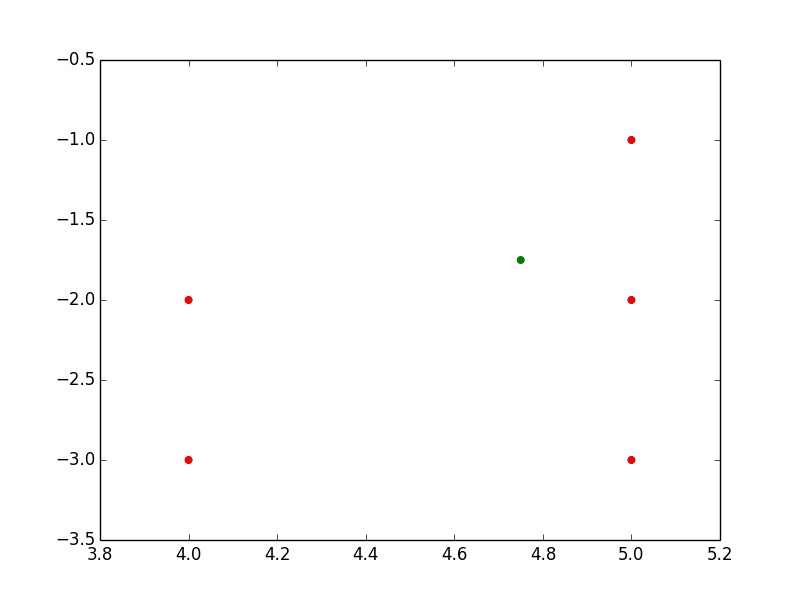
\includegraphics[scale=0.5]{figure_3.png}
        \caption{P and Q exactly overlaps thus weights does not play any role.}\label{fig:figure_3.png}
        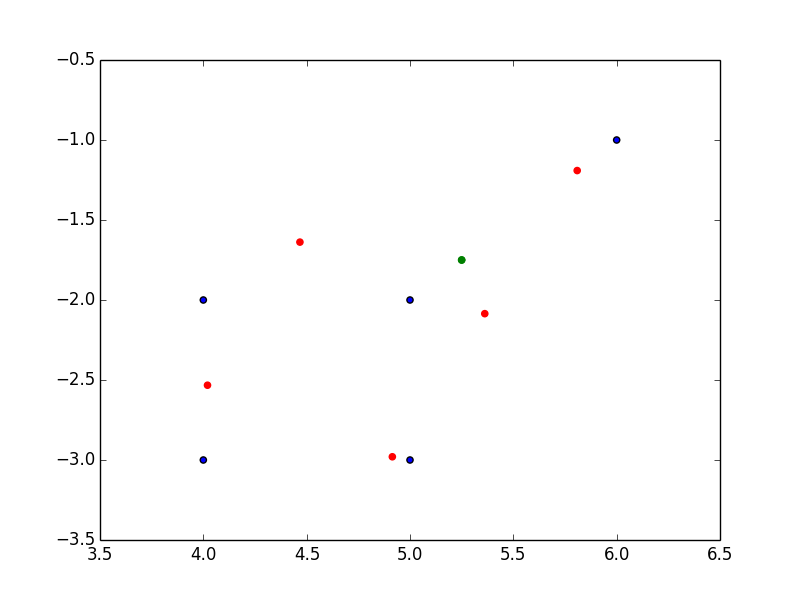
\includegraphics[scale=0.5]{figure_2.png}
        \caption{P and Q could not completely overlap thus weights does play a role in aligning the first vertex.}\label{fig:figure_2.png}
    \end{figure}
\end{enumerate}

\newpage

\section*{Question 2}
References: \cite{Mesh notes}\\
\textbf{Assumptions:}
\begin{enumerate}[label=\alph*.]
    \item
    All faces in the mesh are assumed to be co-planar.
    \item
    All meshes are assumed to the convex in shape.
    
\end{enumerate}

\begin{thebibliography}{1}
\bibitem{Mesh notes}
Mesh Structure Lecture Notes. Geo modelling and Analysis Resource. Musabbir Majeeb \url{https://lms.habib.edu.pk/access/content/group/fe4d011d-731c-4b4c-8570-81d8eaecd21f/modified.pdf} 
\bibitem{rigid body}
Eggert, D. W., Lorusso, A., \& Fisher, R. B. (1997). Estimating 3-D rigid body transformations: a comparison of four major algorithms. Machine vision and applications, 9(5-6), 272-290. \url{http://graphics.stanford.edu/~smr/ICP/comparison/eggert_comparison_mva97.pdf} 

\end{thebibliography}

\end{document}

